\chapter{\huge Algoritmo Metropolis}

\textit{Il Metropolis è l'algoritmo più influenziale fra quelli appartenenti alla classe dei metodi Monte Carlo. Supportato da un'ampia teoria sulle catene di Markov~\cite{due}, questo algoritmo costituisce uno strumento fondamentale per la scienza della computazione.}

\textit{In questa sezione si propone di sviluppare un algoritmo Metropolis per simulare un oscillatore armonico quantistico e confrontare i risultati numerici con la teoria.}
\\

Il metodo Metropolis~\cite{quattro} nasce dalla necessità pratica di dover generare numeri casuali distribuiti con una densità di probabilità $p(x_1,...,x_d)$, che non necessariamente fattorizza. Sia il vettore $\phi = (x_1,...,x_d)$ uno stato dell'ensemble, che vogliamo generare. L'algoritmo consiste nel partire da uno stato iniziale $\phi_0$, e sostituire iterativamente uno stato vecchio con uno nuovo, in maniera tale da ottenere la distribuzione corretta nel limite di un gran numero di iterazioni. La distribuzione che viene raggiunta all'equilibrio è indipendente dallo stato iniziale $\phi_0$. Una volta che tale distribuzione è stata raggiunta, l'applicazione ripetuta dell'algoritmo mantiene il sistema all'interno dello stesso ensemble. In altre parole, la distribuzione desiderata costituisce l'unico punto fisso dell'algoritmo.

Due condizioni importanti devono essere soddisfate per poter applicare il Metropolis: Ergodicità e bilancio dettagliato. La condizione di bilancio dettagliato afferma che le probabilità di transizione $W(\phi_1\rightarrow\phi_2)$ e $W(\phi_2\rightarrow\phi_1)$ rispettano l'equazione $$p(\phi_1)W(\phi_1\rightarrow\phi_2) = p(\phi_2)W(\phi_2\rightarrow\phi_1)$$
L'ergodicità invece richiede che ogni stato dell'ensemble possa essere raggiunto in un numero finito di steps.

Dato uno stato iniziale $\phi_1$, un'iterazione dell'algoritmo consiste delle seguenti istruzioni:
\begin{itemize}
    \item generare casualmente un nuovo candidato $\phi'$
    \item calcolare $\Delta S = -\log(p(\phi')/p(\phi_1))$
    \item se $\Delta S < 0$ impostare il nuovo stato $\phi_2=\phi'$
    \item se $\Delta S > 0$ accettare il nuovo candidato con probabilità $p(\phi')/p(\phi_1)$, altrimenti mantenere $\phi_1$
    \item passare all'iterazione successiva
\end{itemize}
L'algoritmo Metropolis tuttavia presenta alcuni svantaggi, tra i quali il fatto che quando si raggiunge la distribuzione d'equilibrio, gli stati successivi sono in genere molto correlati. Se si vuole ottenere un unbiased sample di stati $\phi_i$ si possono quindi trascurare un numero $\tau_d$ di stati prima di passare a quello successivo. Il numero di steps $\tau_d$ viene denominato tempo di decorrelazione ed è dell'ordine di $\xi^2$, dove $\xi$ è una tipica distanza di correlazione del sistema. Ciò è dovuto al fatto che il Metropolis aggiorna gli stati localmente in maniera casuale. L'agoritmo consiste quindi nell'eseguire un random walk attraverso lo spazio delle configurazioni, il che richiede $\xi^2$ passaggi per effettuare uno spostamento di una distanza $\xi$ in una certa direzione.

\section{Oscillatore Armonico}
Il sistema è costituito da una particella che si muove in uno spazio unidimensionale e in un reticolo temporale finito di passo $a$ e lunghezza $N$ con condizioni di periodicità al contorno. Le variabili del sistema sono quindi le coordinate $x_t$ della particella ai vari istanti di tempo $t$, con la condizione $x_N \equiv x_0$. La particella interagisce inoltre con un potenziale armonico della forma $$V(x) = \frac{m}{2}\omega^2 x^2$$

In meccanica quantistica la stima di un osservabile può essere estratta dalle funzioni di correlazione del sistema~\cite{otto}.
Si calcola quindi il correlatore delle variabili $l$-esima e $k$-esima $\langle x_lx_k\rangle$, definito dalla formula
$$\langle x_lx_k\rangle=\frac{\int Dx\ x_lx_ke^{-S_E}}{\int Dx\ e^{-S_E}}$$
Calcolare il correlatore significa calcolare un \textit{path integral}~\cite{sette} usando come ampiezza di probabilità il fattore $e^{-S_E}$. Il ruolo dell'algoritmo Metropolis è dunque quello di generare configurazioni del sistema con distribuzione di ampiezza di probabilità $e^{-S_E}$.
\\

Dopo aver ottenuto una stima per il correlatore delle variabili $x_l$ e $x_k$ per ogni combinazione di $(l,k)$, si ricavano infine i valori di $\Delta E=(\tilde{E}_1-\tilde{E}_0)$ e dell'elemento di matrice $W=\langle\tilde{E}_0|\hat{x}|\tilde{E}_1\rangle$ invertendo la relazione
\begin{center}
\small
$\langle x_l x_k\rangle = 2|\langle\tilde{E}_0|\hat{x}|\tilde{E}_1\rangle|^2\exp\left(-\frac{Na}{2}(\tilde{E}_1-\tilde{E}_0)\right)\cosh\left[a\left(\frac{N}{2}-|l-k|\right)(\tilde{E}_0-\tilde{E}_1)\right]$.
\end{center}

\subsection{Azione e Termalizzazione}

Partendo da uno stato $\phi_0$ casuale, è necessario lasciare del tempo affinchè sistema si porti alla $pdf$ di equilibrio. Tale processo, denominato termalizzazione, richiede in questo caso non più di 500 cicli di Metropolis, eseguiti i quali sarà possibile estrarre le configurazioni con la distribuzione desiderata. Come condizione iniziale si possono inizializzare tutte le variabili a zero (cold start) oppure a valori random (hot start).
\begin{figure}[H]
\centering
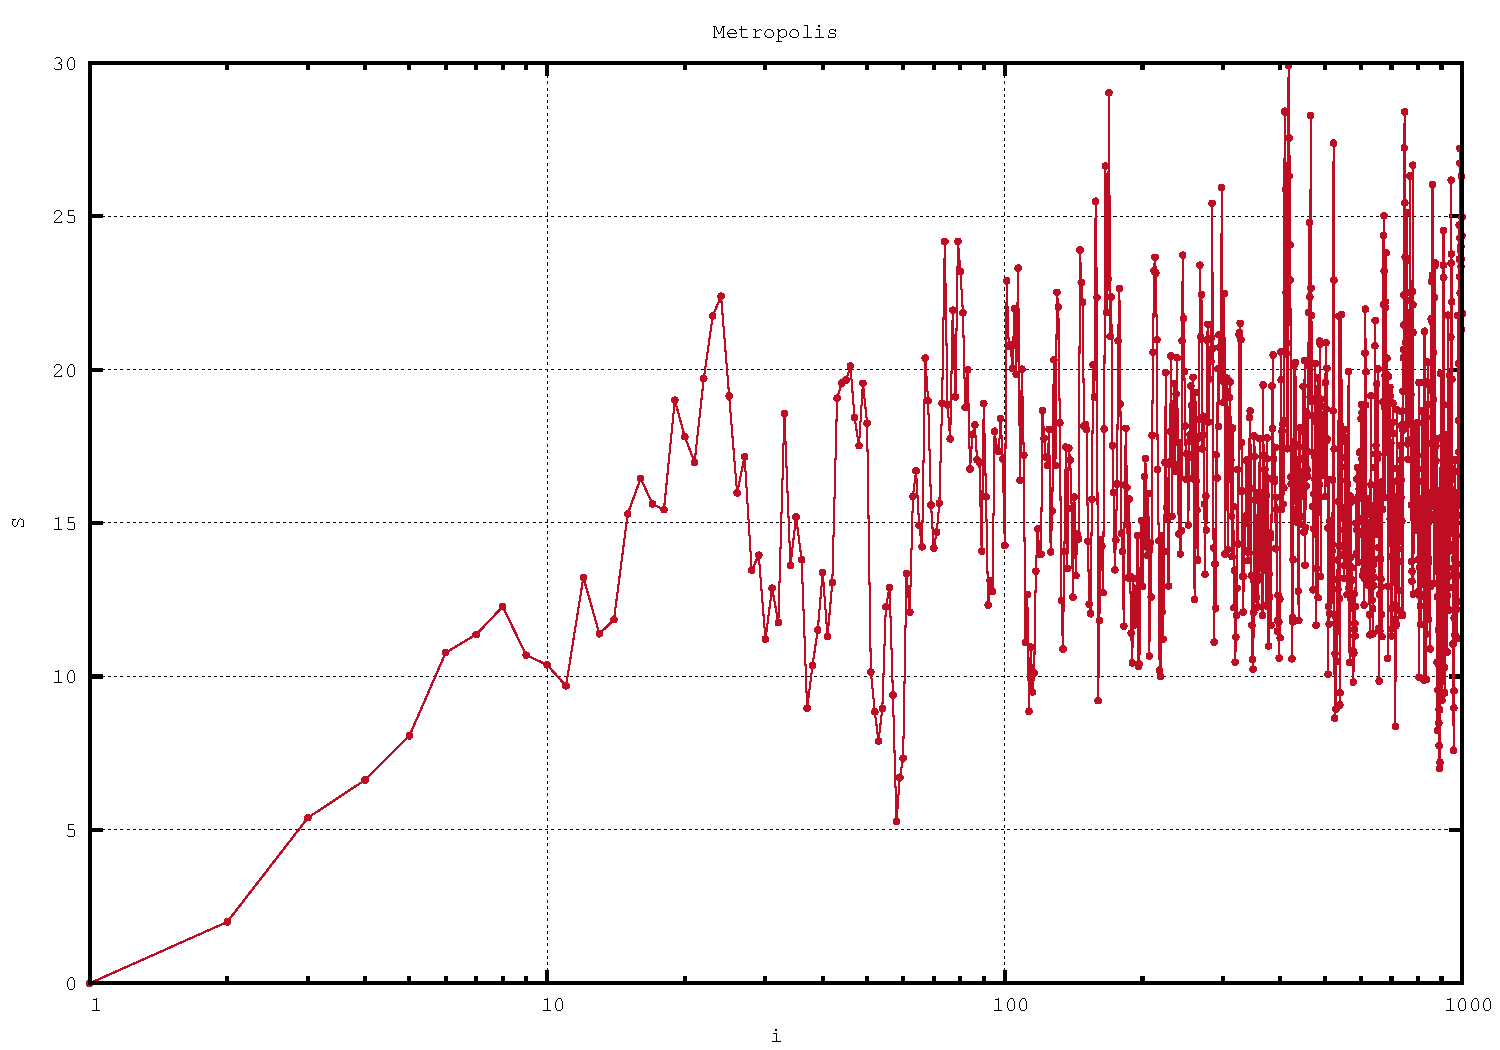
\includegraphics[width=0.5\textwidth]{action1}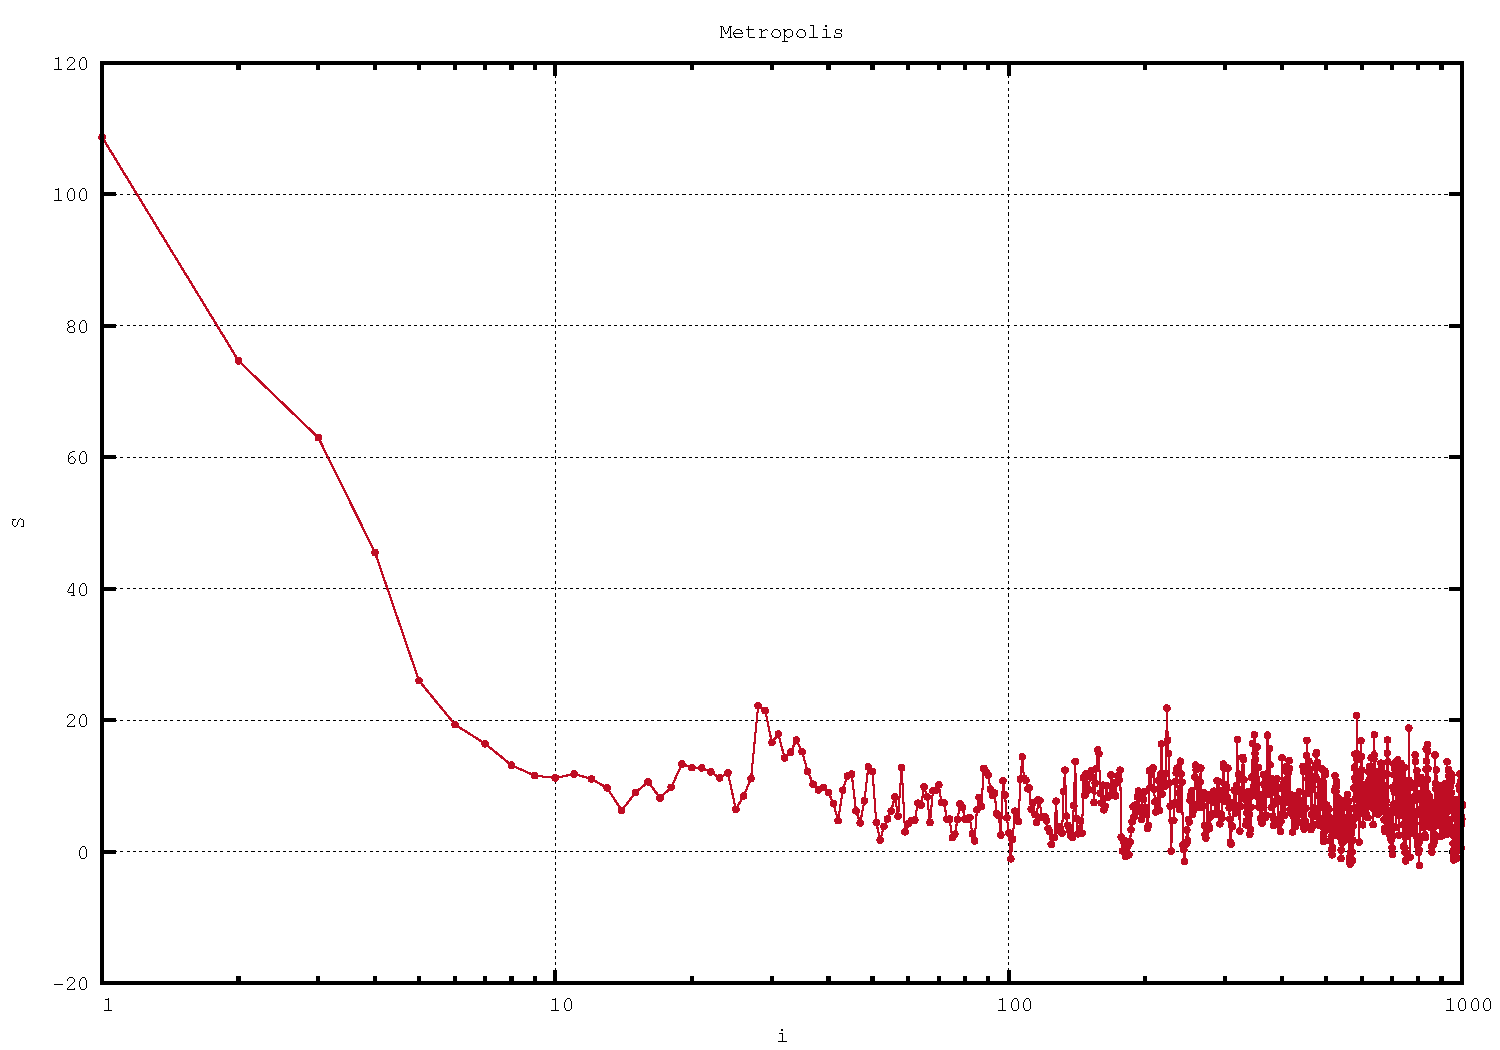
\includegraphics[width=0.5\textwidth]{action2}
\caption{Cold start e hot start}
\label{fig:action}
\end{figure}
Per il calcolo dell'azione euclidea si usa la formula
$$S = a\displaystyle\sum\limits_{i=0}^{N-1} \mathcal{L}(x_{i},x_{i+1})$$
dove
$$\mathcal{L}(x_{i},x_{i+1}) = \frac{m}{2}\left(\frac{x_{i}-x_{i+1}}{a}\right)^{2}-\frac{1}{2}V(x_{i})-\frac{1}{2}V(x_{i+1})$$
Tuttavia, per calcolare $\Delta S = S'-S$ si può tenere presente il fatto che ad ogni estrazione solo una variabile di sistema viene modificata e quindi tutti i termini delle due sommatorie che non contengono quella variabile si elidono nella differenza. Pertanto si utilizza la formula ridotta
\begin{eqnarray*}
 \Delta S_i &=& a[\mathcal{L}(x_{i-1},x'_{i})+\mathcal{L}(x'_{i},x_{i+1})-\mathcal{L}(x_{i-1},x_{i})-\mathcal{L}(x_{i},x_{i+1})]\\
   &=& \tfrac{m}{a}[(x_{i}-x'_{i})(x_{i+1}+x_{i-1})+(x'^2_i-x^2_i)]+aV(x'_i)-aV(x_i)
\end{eqnarray*}

È facile verificare che l'algoritmo e i risultati possono essere resi indipendenti dal fattore di reticolo $a$ se si ridefiniscono propriamente i parametri del problema, il che è equivalente a porre $a=1$.

\subsection{Autocorrelazione}

Si studia ora la correlazione tra configurazioni generate a step consecutivi dell'algoritmo per ottenere una stima del tempo di decorrelazione $\tau_d$ del sistema. Tale dipendenza fra elementi della catena viene anche denominata \textit{autocorrelazione}.

La formula per il correlatore di due stime dell'osservabile $O$ calcolate da stati estratti a istanti di tempo distanti $\tau$ è
$$R(\tau)=\frac{\langle O_iO_{i+\tau}\rangle-\langle O_i\rangle^2}{\langle O_i^2\rangle-\langle O_i\rangle^2}=\frac{\frac{1}{n-\tau}\sum\limits_{i=0}^{n-\tau}O_iO_{i+\tau}-\langle O_i\rangle^2}{\langle O_i^2\rangle-\langle O_i\rangle^2}$$

Il grafico dell'autocorrelazione $R(\tau)$ per l'osservabile $O(|l-k|)=\langle x_lx_k\rangle$ evidenzia la perdita esponenziale di correlazione nel segnale.
\begin{figure}[H]
\centering
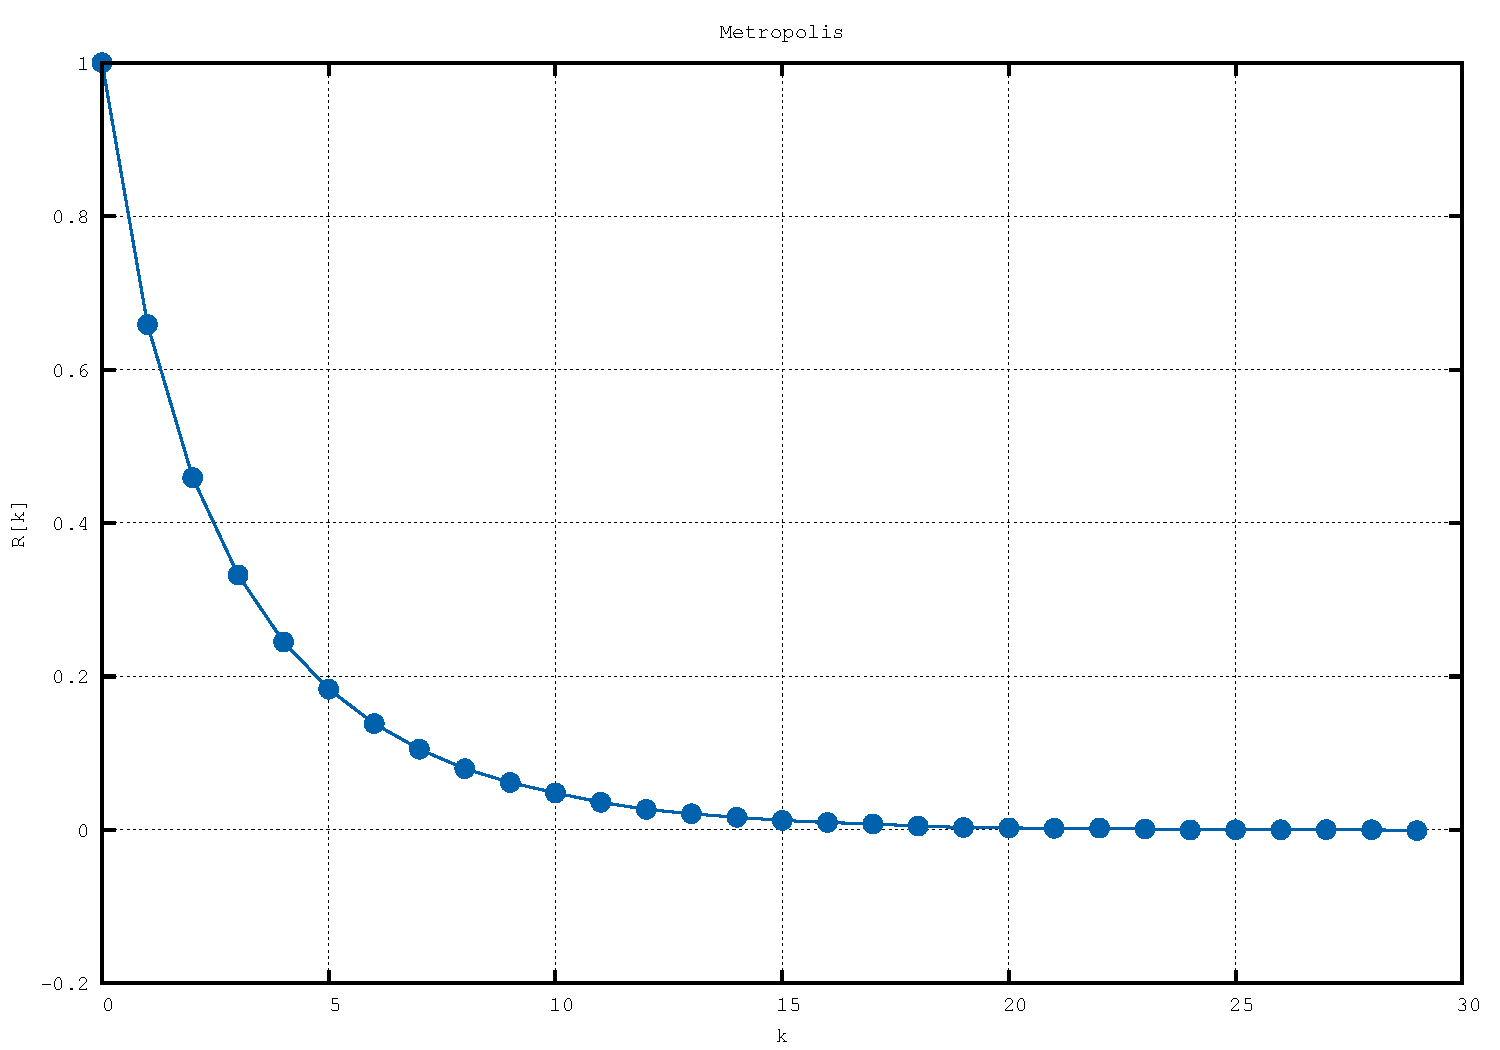
\includegraphics[width=\textwidth]{autocorrelation}
\caption{Autocorrelazione dell'osservabile $\langle x_lx_k\rangle$ per $|l-k|=1$}
\label{fig:autocorrelation}
\end{figure}
Il tempo di decorrelazione $\tau_d$ è dell'ordine delle unità ($\sim3$) e quindi, per $\tau>5\tau_d$ il segnale può essere considerato praticamente scorrelato.

\subsection{Funzioni di Correlazione}

Si calcola numericamente l'integrale $\int Dx \ x_lx_ke^{-S_E}$ applicando i metodi Monte Carlo e Metropolis in congiunzione. Affinchè le configurazioni utilizzate siano statisticamente indipendenti, si raggruppano i sample in $bin$ e si utilizza l'insieme delle medie su ogni $bin$ come sample di configurazioni per il calcolo MC. In questo modo, se la dimensione dei $bin$ è molto maggiore di $\tau_d$, la media sul $bin$ attenua considerevolmente gli effetti di correlazione e perciò il nuovo sample può essere considerato statisticamente unbiased.

La media di un generico osservabile $O$ calcolata in questo modo è analiticamente uguale a quella calcolata per mezzo del sample completo di ogni elemento estratto. La varianza sui valori medi, tuttavia, differisce dalla varianza semplice di un termine proporzionale alla covarianza fra le variabili.

\begin{figure}[H]
\centering
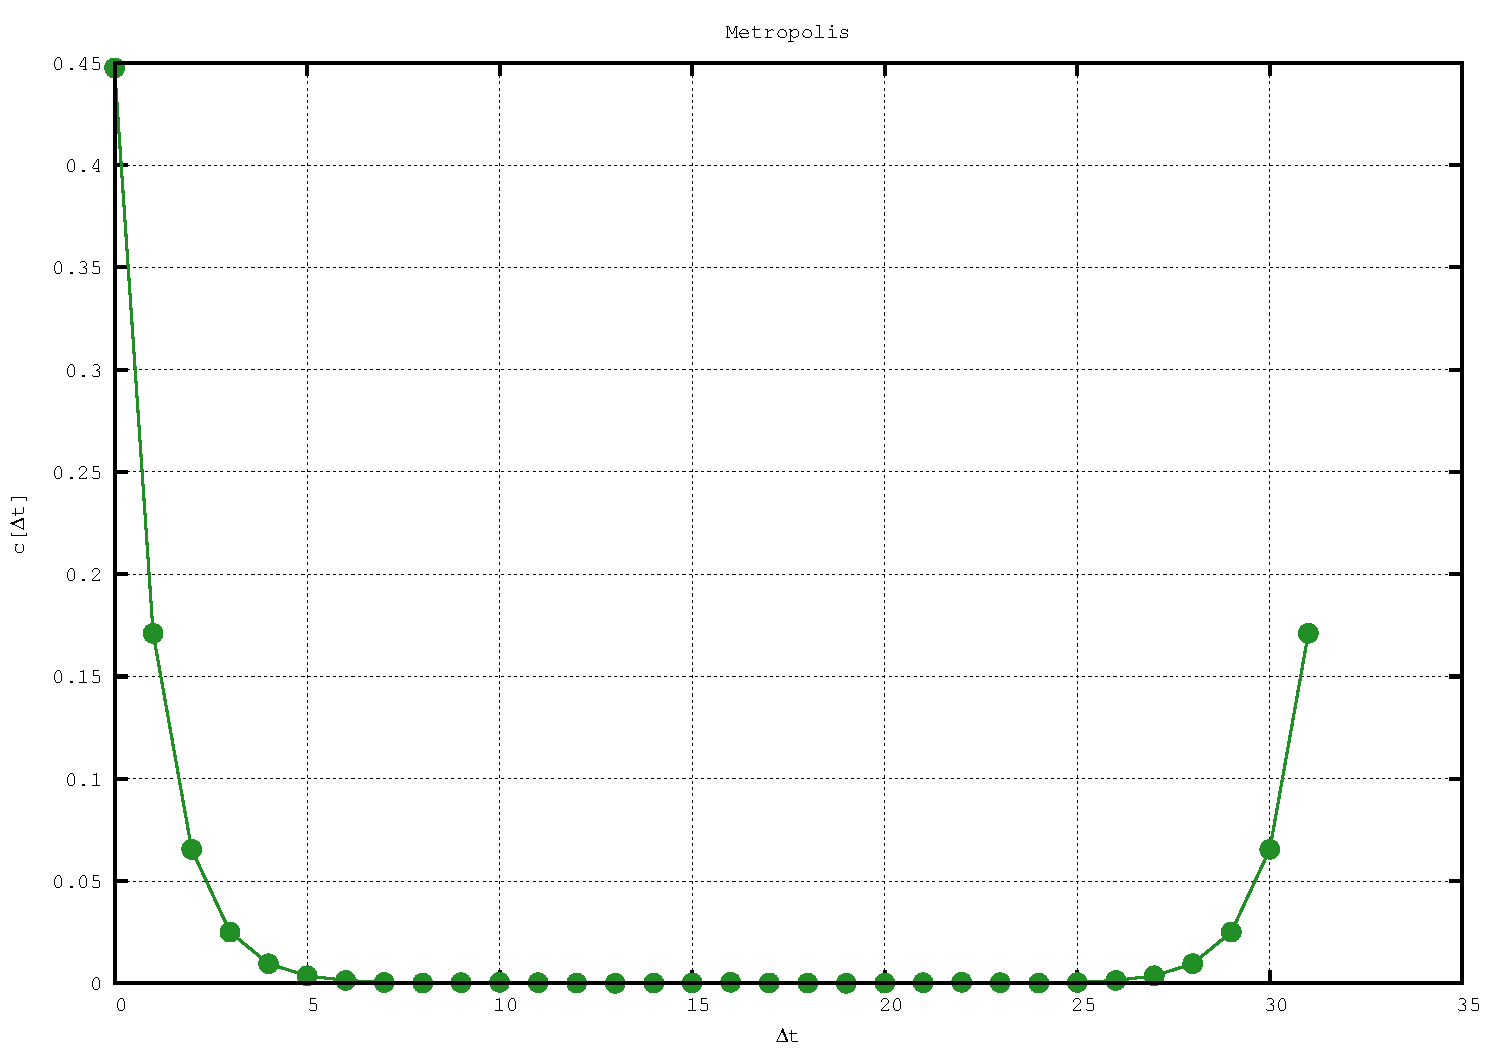
\includegraphics[width=\textwidth]{correlation}
\caption{L'andamento del correlatore delle coordinate in funzione della loro separazione nel reticolo temporale è quello di un coseno iperbolico centrato in $|l-k|=\tfrac{N}{2}$.}
\label{fig:correlation}
\end{figure}

\subsection{Calcolo di Grandezze Quanto-Meccaniche Secondarie}

Come anticipato nell'introduzione sull'oscillatore armonico, è ora possibile ricavare stime di grandezze quanto-meccaniche secondarie direttamente dai valori delle funzioni di correlazione del sistema $\langle x_lx_k\rangle$. Le varianze sui valori medi sono calcolate attraverso la tecnica \textit{cluster jackknife}.
\\

Sia $o_i$ la stima semplice dell'osservabile $O$ allo step $i$. La tecnica \textit{cluster jackknife} consiste nel ricavare le grandezze derivate $o^i$ (\textit{clusterization}), definite come $$o^i=\langle o\rangle+\frac{\langle o\rangle-o_i}{N_{bin}-1}$$ dove $N_{bin}$ indica il numero totale di $bin$. Nel caso in esame la grandezza $O$ è il correlatore calcolato nella sezione precedente.

Data una funzione $f=f(o)$, si definiscono $f^i=f(o^i)$ e $\langle f\rangle=f(\langle o\rangle)$. Si ottiene allora $$\sigma^2_f=\frac{N_{bin}-1}{N_{bin}}\sum\limits_i(f^i-\langle f\rangle)^2$$
I valori utilizzati per i parametri del sistema sono $N=32$, $\hbar=1$, $a=1$, $\omega=1$, $m=1$ e i valori ottenuti sono
\begin{eqnarray*}
\Delta E&=&0.9629359930\pm0.0057513054\\
W&=&0.6679253933\pm0.0071617466
\end{eqnarray*}

In figura \ref{fig:histogram} si nota come l'errore statistico coincida con una buona approssimazione con quello stimato dal \textit{cluster jackknife}.

\begin{figure}[H]
\centering
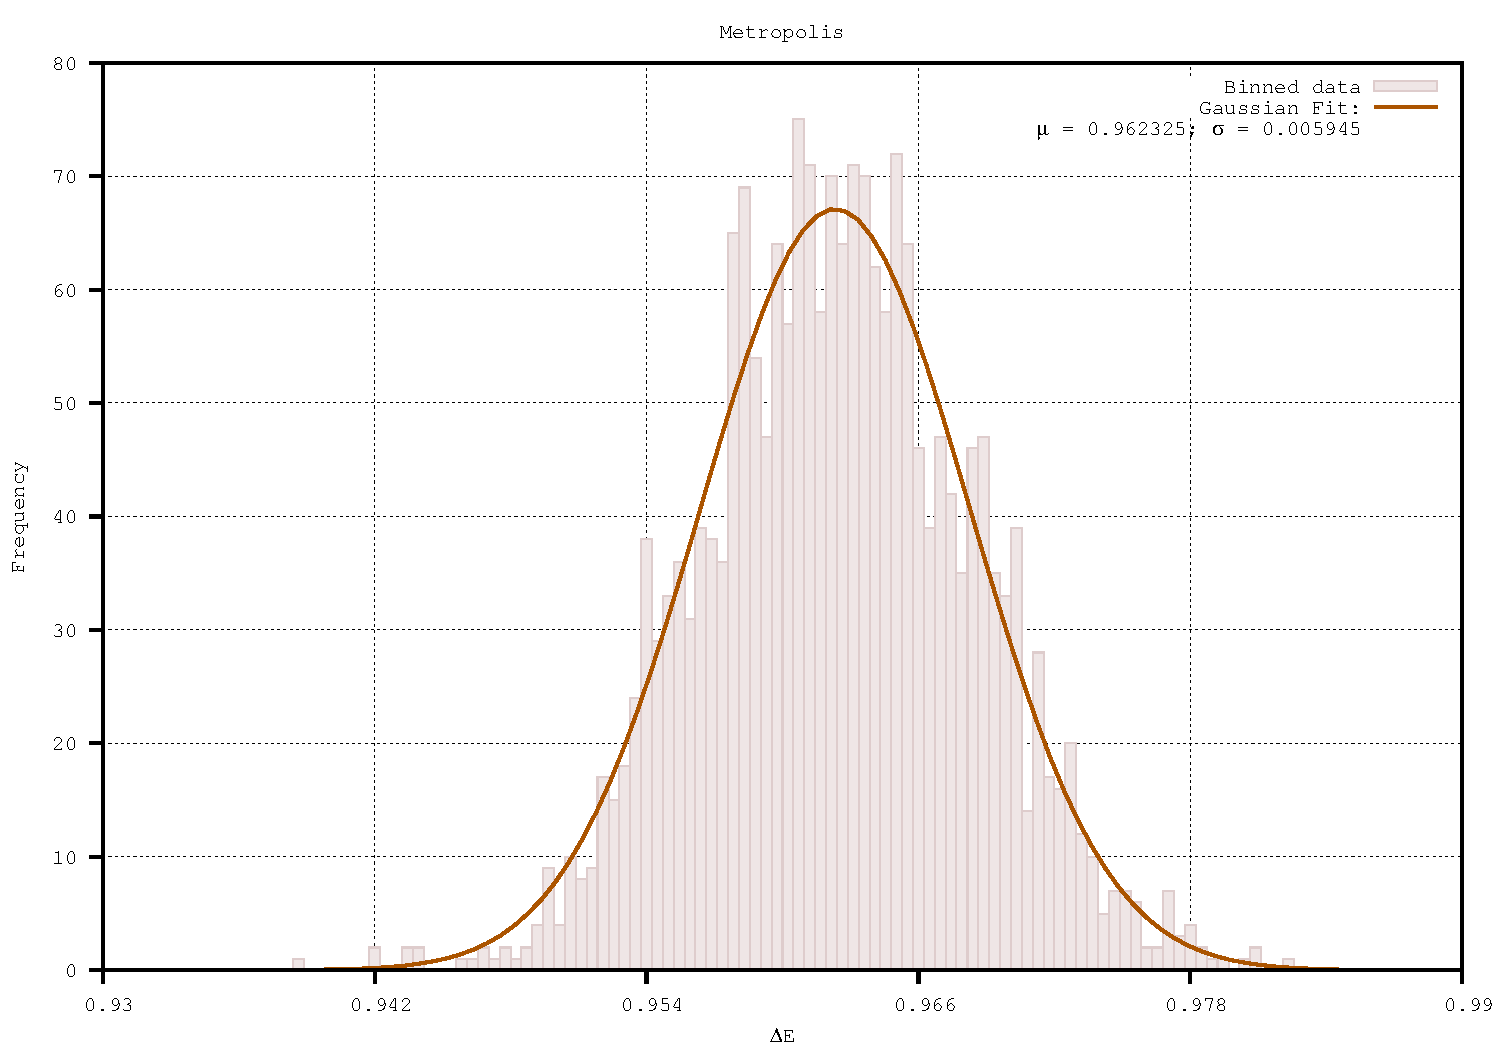
\includegraphics[width=0.7\textwidth]{histogram}
\caption{Distribuzione di $\Delta E$ a fissato numero di sweeps}
\label{fig:histogram}
\end{figure}
\begin{figure}[H]
\centering
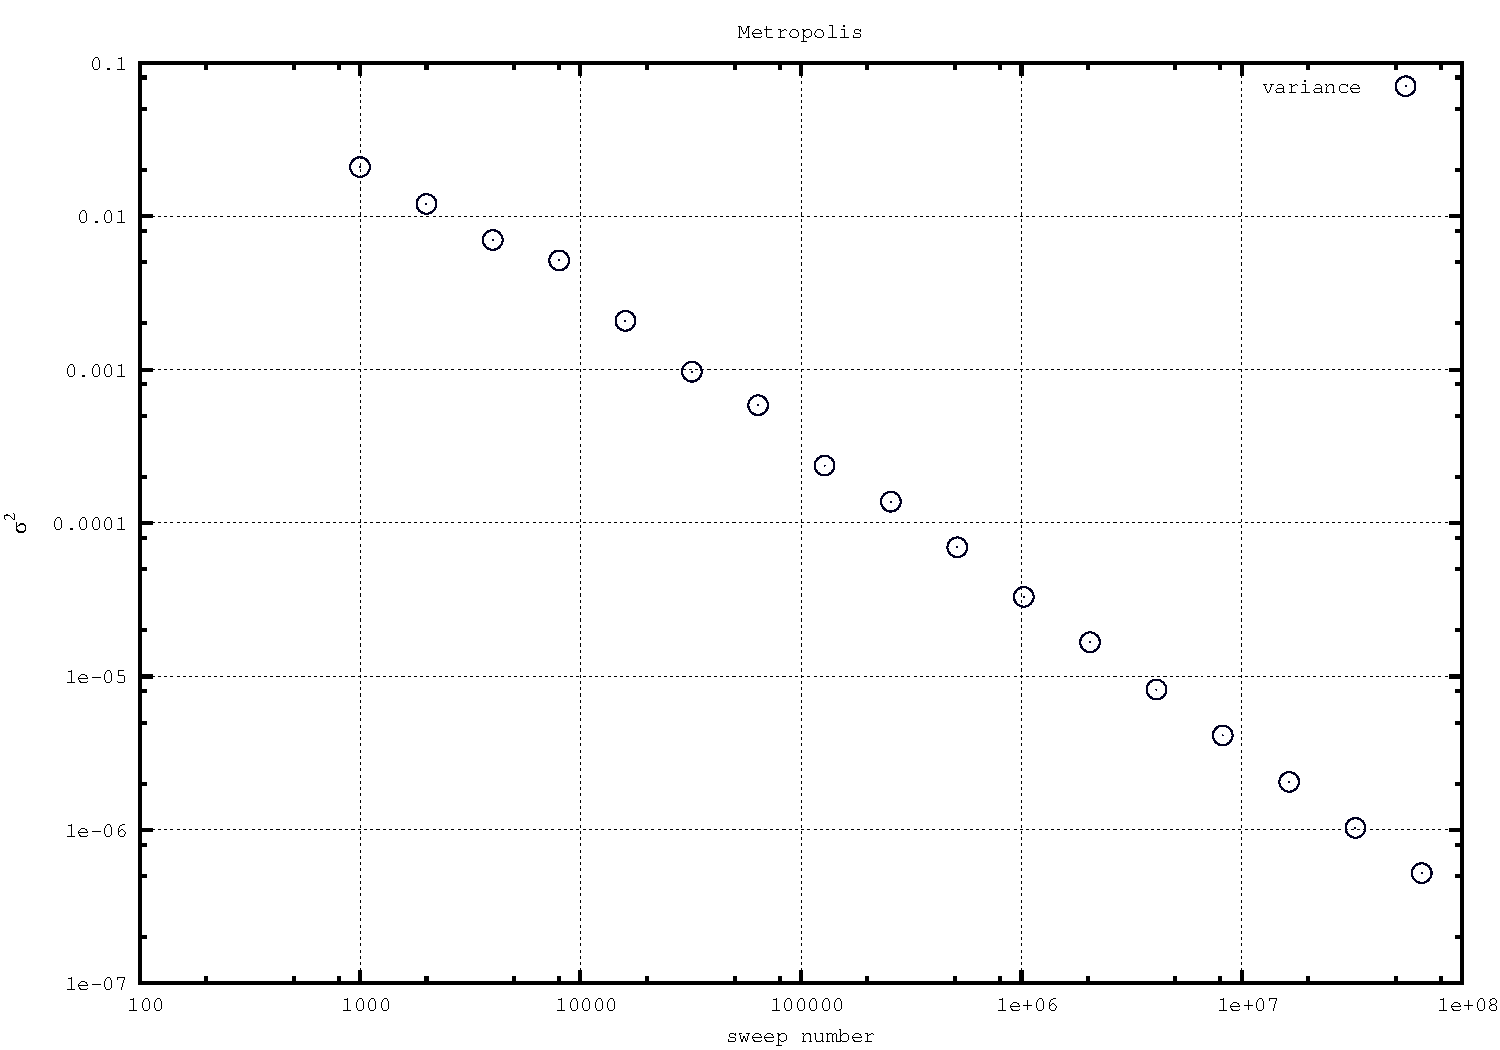
\includegraphics[width=0.7\textwidth]{variance}
\caption{Varianza di $\Delta E$ in funzione del numero di sweeps}
\label{fig:variance}
\end{figure}

